\documentclass[12pt,a4paper,fleqn]{article}
\usepackage{rmpackages}																% usual packages
\usepackage{rmtemplate}																% graphic charter
\usepackage{rmexocptce}																% for DS with cptce eval

%\cfoot{} 													% if no page number is needed
%\renewcommand\arraystretch{1.5}		% stretch table line height

\newcommand{\ritem}{\refstepcounter{enumi}\item[$\star$ \theenumi .]}

\begin{document}

\begin{header}
Activité -- Compter des entités chimiques
\end{header}

Quand on achète des pâtes, on ne les achète pas à l'unité : on en prend un paquet.
De la même façon, le lycée commande des ramettes de papier qui contiennent chacune 500 feuilles.

En chimie, on manipule des échantillons de matière qui contiennent un nombre réellement astronomique d'atomes, de molécules ou d'ions.
Les chimistes ont donc trouvé une méthode pour simplifier le comptage des entités contenues dans un échantillon : la \textbf{mole}.
L'objectif de cette activité est d'aborder cette nouvelle façon de compter des entités chimiques.

\section*{Quelle est la masse d'une molécule ?}

\begin{enumerate}
\item Un atome d'oxygène a une masse de \unit{2\dcoma 66 \times 10 ^{-26}}{kg}.
Une molécule de dioxygène $\dioxygene$ est formée de deux atomes d'oxygène.
Calculer la masse d'une molécule de dioxygène.
\end{enumerate}
\begin{multicols}{2}
\begin{enumerate}[resume]
\item Calculer la masse $m_\methane$ d'une molécule de méthane $\methane$.

\ritem Calculer la masse $m_\mathrm{benz}$ d'une molécule de benzaldéhyde, un liquide à l'odeur d'amande amère, dont le schéma de Lewis est représenté ci-contre.
\end{enumerate}

\begin{center}
\chemfig[angle increment=30, atom sep=20pt]{[:30]C(-[6]H)*6(-C(-H)=C(-H)-C(-C(=[3]\lewis{13,O})(-[-1]H))=C(-H)-C(-H)=)}
\end{center}
\end{multicols}

\paragraph{Données :}
\begin{itemize}
\item[•] masse d'un atome d'hydrogène : $m_\mathrm{H} = \unit{1\dcoma 67 \times 10 ^{-27}}{kg}$ ;
\item[•] masse d'un atome de carbone : $m_\mathrm{C} = \unit{1\dcoma 99 \times 10 ^{-26}}{kg}$ ;
\item[•] masse d'un atome d'oxygène : $m_\mathrm{O} = \unit{2\dcoma 66 \times 10 ^{-26}}{kg}$.
\end{itemize}

\section*{Compter des particules}

\begin{multicols}{2}
\begin{enumerate}
\setcounter{enumi}{3}
\item La masse d'un seau rempli de balles de tennis est de \unit{3600}{g}, chaque balle a une masse de \unit{57}{g}.
Déterminer le nombre de balles dans le seau.
Comment expliquer l'écart par rapport au nombre indiqué sur le seau ?

\item La masse d'une règle en aluminium est $m_\mathrm{règle} = \unit{0\dcoma040}{kg}$ et celle d'un atome d'aluminium est $m_\mathrm{Al} = \unit{4\dcoma48 \times 10^{-26}}{kg}$.
Calculer le nombre d'atomes d'aluminium qui constituent la règle.

\ritem Un échantillon de masse $m$ est constitué d'entités chimiques identiques de masse $m_\mathrm{entité}$.
Donner la formule littérale permettant de calculer le nombre $N$ d'entités contenues dans cet échantillon. 
\end{enumerate}

\begin{center}
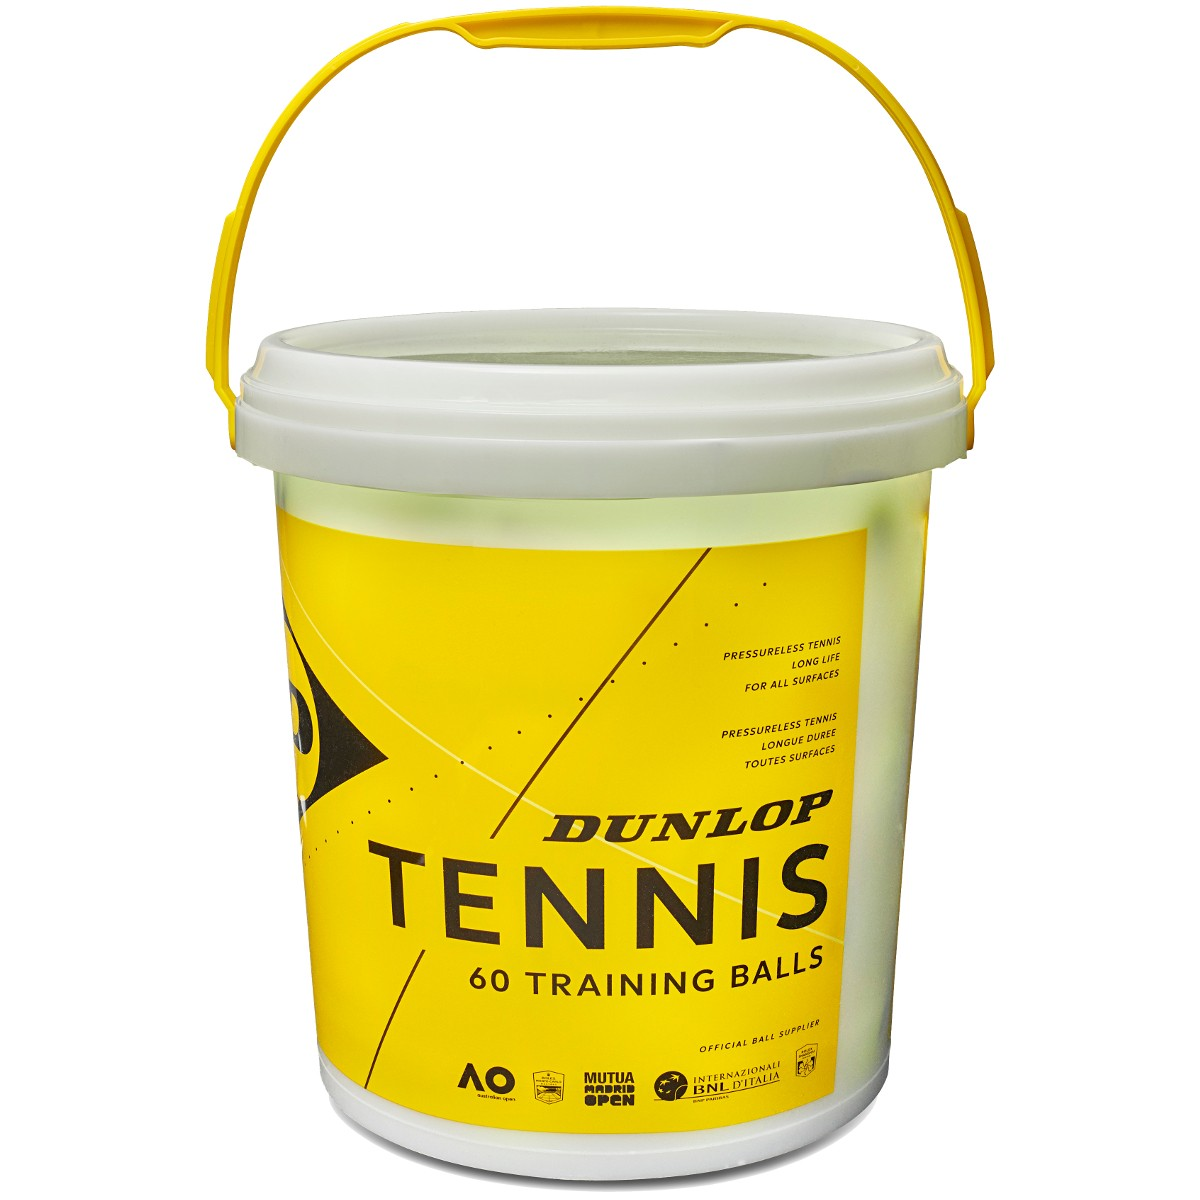
\includegraphics[height=200pt]{images/seau_de_balles.jpg}
\end{center}
\end{multicols}

\section*{Quantité de matière}

\begin{enumerate}
\setcounter{enumi}{6}
\item Regarder la vidéo \href{https://youtu.be/\_kosdfe79OU}{https://youtu.be/\_kosdfe79OU} puis répondre au quiz

\href{https://www.quiziniere.com/\#/Exercice/EYWZ56}{https://www.quiziniere.com/\#/Exercice/EYWZ56}

%\href{https://www.quiziniere.com/\#/Exercice/QG6QBO}{https://www.quiziniere.com/\#/Exercice/QG6QBO}.
\label{quest:quiz}
\end{enumerate}

\section*{Autant de molécules d'eau dans un dé à coudre que d'étoiles dans l'Univers ?}

\begin{multicols}{2}
\begin{center}
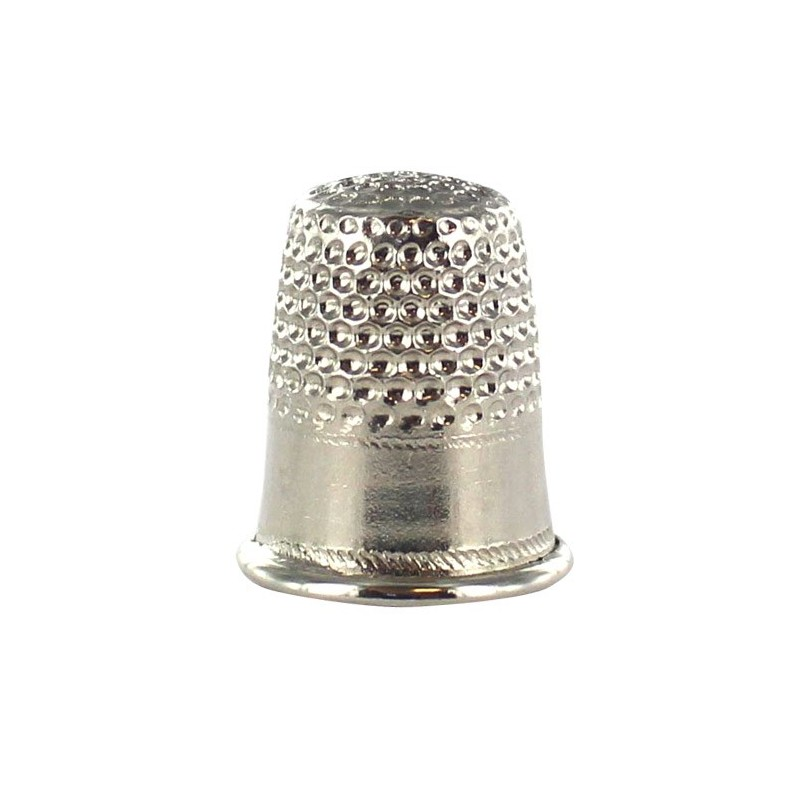
\includegraphics[angle=180,width=\linewidth]{images/de_a_coudre.jpg}

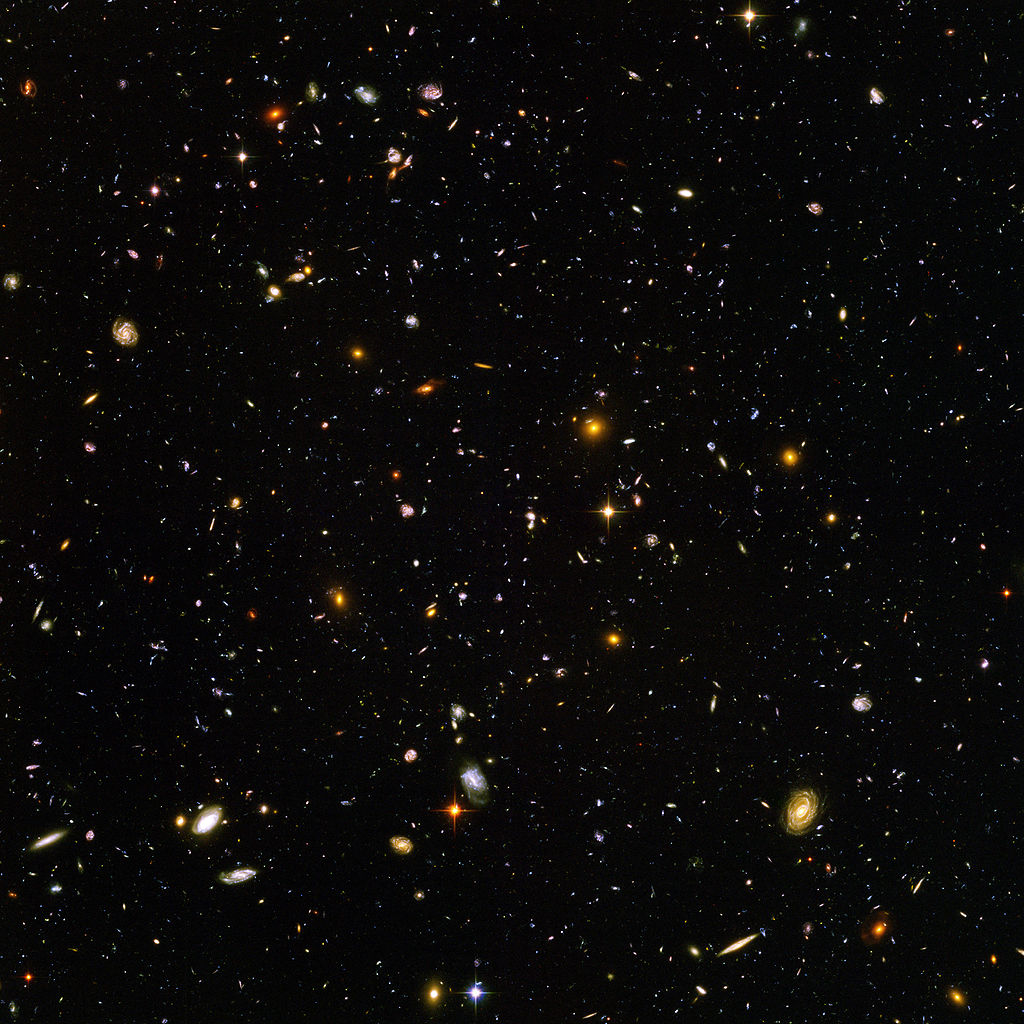
\includegraphics[width=\linewidth]{images/hubble_ultra_deep_field.jpg}
\end{center}
\end{multicols}

Un dé à coudre peut contenir environ \unit{3}{g} d'eau.

\begin{enumerate}[resume]
\item Rappeler la formule chimique de l'eau.

\ritem Calculer la masse d'une molécule d'eau en utilisant les valeurs données précédemment.

\ritem Calculer le nombre de molécules contenues dans un dé à coudre.

\ritem Comparer ce nombre au nombre de grains de sable sur Terre (cf. vidéo de la question~\ref{quest:quiz}).

\ritem Et au nombre d'étoiles dans l'Univers ?
On estime qu'il y a environ 250 milliards ($250\times10^9$) de galaxies dans l'Univers et que chacune contient environ 400 milliards ($400\times10^9$) d'étoiles.
\footnote{
On parle ici de l'Univers observable.
Plus de détails sur la manière dont sont réalisées ces estimations ici : \href{https://scienceetonnante.com/2012/07/23/y-a-t-il-plus-detoiles-dans-lunivers-que-de-grains-de-sable-sur-terre/}{https://scienceetonnante.com/2012/07/23/y-a-t-il-plus-detoiles-dans-lunivers-que-de-grains-de-sable-sur-terre/}.
}

\ritem Calculer la quantité de matière d'eau contenue dans le dé à coudre.
\end{enumerate}

\end{document}

\section*{Conversation fictive entre Avogadro et Ampère}

Monsieur Ampère,

Je souhaite vous  faire part d'une  découverte  qui  a bien  simplifié  ma  vie  et  qui,  si  vous  m'en  croyez, pourrait  bien simplifier  la  vôtre.

Professeur de chimie, j'ai l'habitude de donner à mes étudiants des exercices destinés à éveiller leur jeune intelligence.
Il y a quelques semaines, je leur proposai l'énoncé suivant : 

\og On fait réagir 8 grammes de dihydrogène avec 64 grammes de dioxygène.
Il se forme de l'eau.
Sachant que 4 grammes de dihydrogène contiennent 2 408 854 000 000 000 000 000 000 molécules et que 64 grammes de dioxygène contiennent 1 204 426 000 000 000 000 000 000 molécules, quel sera le nombre de molécules d'eau formées ? \fg{}
Je me désespérais des résultats : même les meilleurs élèves s'égaraient dans les calculs monstrueux.

Rentrant chez moi un soir, découragé par les résultats de mes élèves sur leur dernier devoir, je me rappelai que ma femme m'avait demandé de lui apporter des œufs.

\og Bonjour, Monsieur l'épicier, pourriez-vous me donner 36 œufs, s'il vous plaît ? \fg{}

\og Bien sûr, Monsieur Avogadro, mais vous pourriez dire 3 douzaines comme tout le monde \fg{}, répondit-il.

Par gourmandise, je lui demandai également 18 crêpes.

\og Une douzaine et demi, Monsieur Avogadro, sans vous commander ! \fg{}, marmonna-t-il.

Chemin faisant, passant devant une poissonnerie, j'entendis une cliente commander 6 douzaines d'huîtres en précisant qu'elle attendait 6 convives.
C'est là, Monsieur Ampère, que devant la porte de la poissonnerie que je fus traversé par le génie. 
\og L'épicier et le poissonnier ont déjà inventé la douzaine pour compter plus facilement leurs crêpes et leurs huîtres et toi tu n’as pas encore inventé la mole .... \fg{}

Ayant pesé avec une extrême précaution 12 grammes de carbone 12 (me méfiant des isotopes), j’entrepris avec un soin non moins extrême de compter les atomes.
Quelques années plus tard, j'y étais parvenu. Il y en avait 602 213 530 000 000 000 000 000 à quelques unités près bien sûr, ce que l'on peut écrire en arrondissant un peu pour la commodité des calculs $6{,}02 \times 10^{23}$.
Je décidai alors que j'appellerai cette collection d'atomes : mole d'atomes de carbone.
Sans mollir, je décidai d'appeler mole de « trucs » tout ce qui contiendrait $6{,}02 \times 10^{23}$ « trucs » identiques.

Je me mis à parler de mole d'atomes de fer, de mole d'électrons, de mole de molécules d'eau, ... et surtout je modifiai la rédaction de mes problèmes :
\og On fait réagir 8 grammes de dihydrogène avec 64 grammes de dioxygène. Il se forme de l'eau. Sachant que 8 grammes de dihydrogène contiennent 4 moles de molécules et que 64 grammes de dioxygène contiennent 2 moles de molécules, quel sera le nombre de mole de molécules d'eau formées ? \fg{}

Et depuis, cher confrère, mes élèves obtiennent d'excellents résultats !

\flushright{Votre dévoué Amédéo AVOGADRO}

\begin{multicols}{2}
\begin{center}
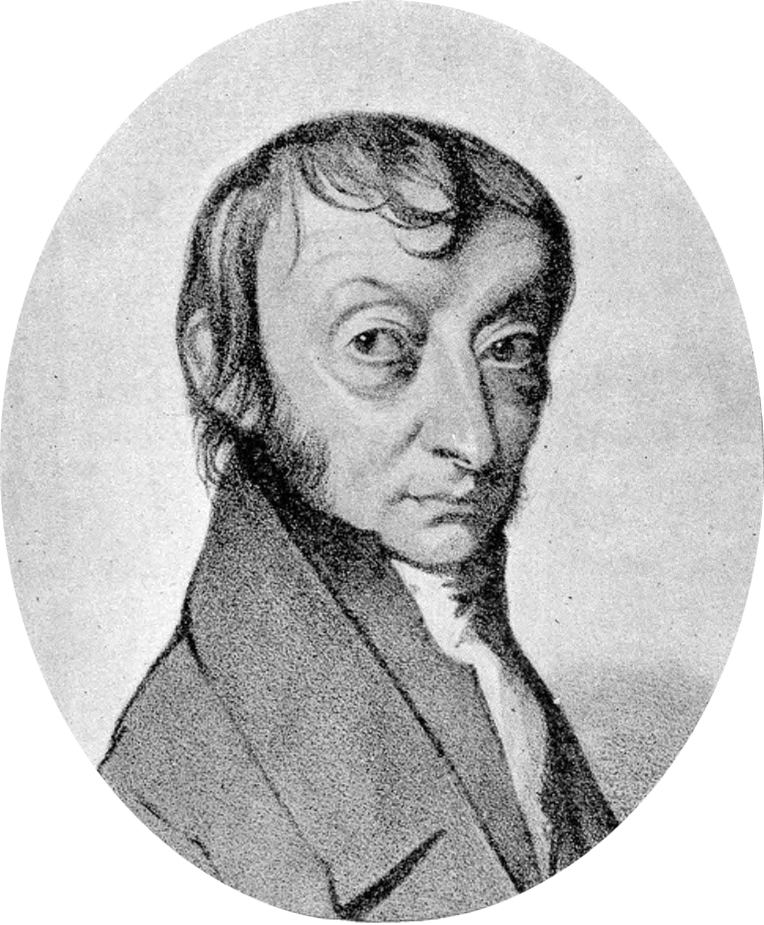
\includegraphics[height=100pt]{images/avogadro_amedeo.jpg}
\end{center}
\begin{center}
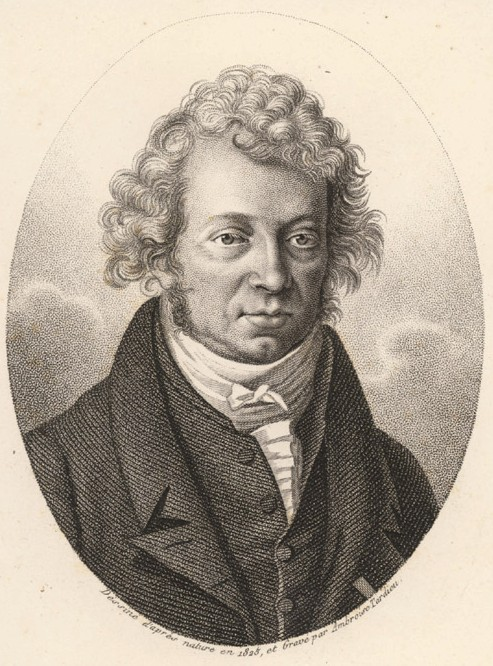
\includegraphics[height=100pt]{images/ampere_andre.jpg}
\end{center}

\end{multicols}